\documentclass[b5paper]{article}

\usepackage[serbianc]{babel}
\usepackage[b5paper, lmargin=0.1\paperwidth, rmargin=0.1\paperwidth, tmargin=0.1\paperheight, bmargin=0.1\paperheight]{geometry} %margins
\usepackage{float}
\usepackage{graphicx}
\usepackage{caption}
\usepackage{subcaption}
\usepackage{hyperref}

\edef\restoreparindent{\parindent=\the\parindent\relax}
\usepackage{parskip}
\restoreparindent

\newcommand{\websource}[1]{\caption*{Преузето са: \href{#1}{#1}}}

\begin{document}

\large

Када причамо о Западу, најчешће је фокус на стању привреде и релативном заостатку Србије. Тема које је мало људи свесно је мрачна страна привредног развоја. У високоиндустријализованим државама света, у порасту је све већи осећај усамљености. Шта је ово проузроковало и постоји ли решење? Колики је удео проблема који је настао природно, а колики вештачки подстакнут? Иако је на оваква питања тешко дати целокупан одговор, усудио бих се да изнесем лични поглед.

Последњих година, у америчкој јавности се све више говори о резултатима истраживања која показују како је број блиских пријатеља становника САД у паду последње три деценије. 1990. године, 40 одсто мушкараца је изјавило да има 10 или више блиских пријатеља, док је 3 одсто изјавило да нема блиских пријатеља. 2020. године, број мушкараца који имају 10 или више блиских пријатеља је опао на 15 одсто, док је број мушкараца који немају блиских пријатеља порастао на 15 одсто\footnote{https://www.americansurveycenter.org/why-mens-social-circles-are-shrinking/}.

1990. године, 28 одсто жена је изјавило да има 10 или више блиских пријатеља, док је 2 одсто изјавило да нема блиских пријатеља. 2020. године, број жена које имају 10 или више блиских пријатеља је опао на 10 одсто, док је број жена које немају блиских пријатеља порастао на 10 одсто.

\begin{figure}[H]
    \centering
    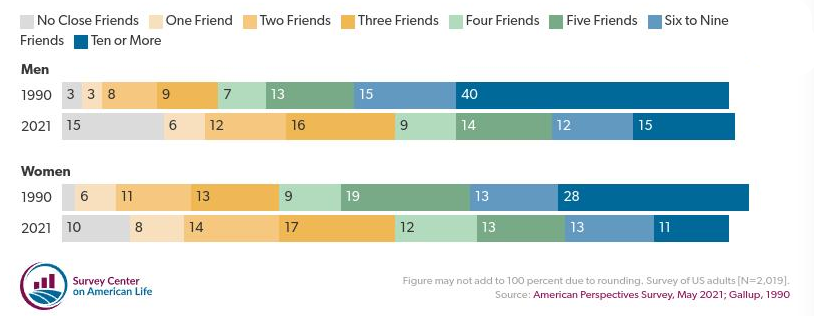
\includegraphics[width=0.7\textwidth,keepaspectratio]{slike/usa_friends.png}
    \websource{https://www.americansurveycenter.org/why-mens-social-circles-are-shrinking/}
\end{figure}

У тренутку писања овог текста, није било доступних упоредивих истраживања на нашим просторима (Србија и бивша Југославија). По једином доступном истраживању над адолесцентима узраста од 13 до 18 година, 37.6 одсто адолесцената је изјавило да има више блиских пријатеља , 53.8 одсто да има неколико блиских пријатеља, 6.9 одсто да има једног блиског пријатеља, док 1.7 одсто нема ниједног блиског пријатеља\footnote{https://www.dps.org.rs/wp-content/uploads/2023/08/Kongres-psihologa-2023-Knjiga-rezimea-2023-08-26.pdf}. Важно је нагласити да због ограничене старосне групе, истаживања нису упоредива.

Други појам присутан у америчкој јавности, како стручној тако и широј је \textit{недостатак додира} (енгл. touch starvation, touch hunger). Под овим појмом, подразумева се стање неспокоја изазвано недостатком физичког додира. Овај појам не потиче из психологије или медицине, већ из колоквијалне употребе. Та чињеница не негира постојање појаве, иако је без истраживања немогуће одредити детаље о распрострањености.

Овај појам је присутан и у домаћој јавности, како у новинама, тако и у блог објавама стручних лица (психијатара и психотерапеута). У жижу јавности појам је дошао са епидемијом корона вируса и закључавањем.

Истраживања су показала везу између задовољавајућег друштвеног живота и бољег здравственог стања и дужег живота\footnote{https://www.ncbi.nlm.nih.gov/pmc/articles/PMC3150158/}. Такође, истраживања су показала како физички додир изазива лучење окситоцина, хормона који утиче на осећање блискости и који подстиче осећање стабилности\footnote{https://elifesciences.org/articles/88215, https://www.health.harvard.edu/mind-and-mood/oxytocin-the-love-hormone}. Да ли је довољно да резултате истраживања прихватимо као такве, или је потребно да у њима потражимо дубљу поуку? Јако важан фактор у доживљају додира јесте и контекст у којем се он десио. Ово нас упућује на дубљи разлог, заснован у психолошким потребама човека.

Алфред Адлер (широј јавности познат по увођену појмова комплекса ниже и више вредности) је сматрао, угледајући се на закључке Чарлса Дарвина, да је због (релативне) физичке немоћи људима неопходан живот у заједници. Људи се рађају са осећањем немоћи које покушавају да савладају целог живота. Ово је, наравно, могуће учинити на здраве и нездраве начине. Као здрав начин, видео је учествовање у заједници. Као неке од нездравих начина, сматрао је одбијање учествовања у заједници, тражење изговора за бежање од изазова и кривљење других за неуспех. Сматрао је да култура има кључни значај у опстанку човека и да је настала из неопходности живота у заједници.

Суштински проблем није само мањи број пријатеља или одсуство физичког додира. Иако као статистички показатељ могу да наговесте негативне промене у друштву, темељнија анализа је неопходна. Прави проблем је све веће осећање отуђености, односно недостатка блискости. На жалост, индивидуализам и отуђеност су особине индустријализованих друштава. Одсуство заједништва за човека није природно, јер је управо живот у заједници обезбедио услове у којима људи данас живе.

Неопходно је нагласити разлику између појмова \textit{самоће} и \textit{усамљености}. Под самоћом подразумевамо стање у којем појединац, без присуства јавности, проводи време. Самоћа омогућава учење, напредак и стваралаштво. Неопходна је за сагледавање света, како спољашњег, тако и унутрашњег. Самоћа је заслужна за сва велика стваралачка дела (како уметничка, тако и техничка) којима се дивимо. Усамљеност је стање непријатности изазване одсусвом блискости и заједништва. Особа која је сама не мора да буде усамљена. Све чешћи случај данас је осећање усамљености, упркос обиљу људи као и садржаја, како из виртуелног, тако и из стварног света.

Тренутна опасност по човечанство је сукоб дугорочног интереса човечанства и краткорочног интереса потрошачког друштва. Дугорочно, човечанство је одрживо искључиво уколико појединци могу да напредују кроз стваралаштво и сарадњу са друштвом. Краткорочно, произвођачи бројних бескорисних производа не би освојили ни тренутак пажње јавности уколико би фокус био на стваралаштву, уместо потрошњи. Још суровија истина је да напредак корпорација управо зависи од подстицања сујете.

Суштина стваралштва је остављање дела које превазилази живот ставароца, као и времена у којем живи. Због тога, стваралаштво је нераскидиво са осећањем заједништва. Насупрот томе, суштина потрошачког друштва је занемаривање било кога осим појединца и његових жеља. Иако на први поглед делује да појединац може да ужива у бесконачној себичности која му се препоручује, резултат је сасвим супротан. Изолованост је неприродна, те не постоји адекватан дугорочан механизам за ношење са оваквим осећањем. Најчешћи ћорсокаци у које води усамљеност су депресија и болести зависности.

Осећај заједништва и стваралштво никада неће бити вредности које ће потрошачко друштво подстицати. Човек којем су на првом месту породица, пријатељи и стваралачки рад никада неће трошити новац на непотребне производе којима су тржни центри преплављени. Али, оваквом системском променом приоритета човечанство залази у ћорсокак. На личном плану, резултат ће бити отуђени и несрећни појединци. На глобалном плану, резултат ће бити нефункционално друштво које није у стању да створи напредак.

Никако не смемо потцењивати ни дигиталне индустрије које директно злоупотребљавају усамљеност. Вероватно најјачу \textit{индустрију усамљености} чине порнографски сајтови. Као наставак, десио се и успон платформе OnlyFans\footnote{Иако ова платформа омогућава приступ плаћеном садржају стваралаца свих струка, 98 одсто садржаја чини порнографија.}, која поред приступа порнографији омогућава и комуникацију са произвођачима порнографије. Иако порнографија није нова појава, бесконачна доступност путем интернета, као и зависност од погрнографије јесу. Иако тема отворене дебате, сматрам да је утицај порнографије штетан.

Такође, многе стриминг платформе омогућавају комуникацију са стримерима. Управо је тај привид блискости узрокован комуникацијом, макар и површном, оно што чини да корисници плате претплату. Стање које ово изазива код чланова публике се назива \textit{парасоцијална веза} (енгл. parasocial relationship). Карактерише је осећање блискости са особом која чак ни не види члана публике као индивидуу. Иако је овде неоспорна велика лична незрелост, уколико је одређена појава иоле масовна, морамо да поставимо питање који су то друштвени фактори који је подстичу.

Као узрок опадања осећаја заједништва, видим комбинацију неповољних животних околности и неадекватног система вредности. За формирање пријатељстава, пре свега је потребно континуирано провођење времена у колективу. Због школовања и посла, људи су све чешће приморани на селидбу. Рад од куће, иако је неоспорно донео предности, значајно онемогућава друштвени живот. Упарено са општим неразумевањем сопствених потреба, за које поред индустрије морамо да окривимо и школски систем, резултат је нарастајуће осећање усамљености.

Ипак, годинама је интересовање за психолошке проблеме човека у порасту. О томе сведочи и брза популарност коју стичу све јавне личности које се одлуче да говоре о датој тематици. Тако највећа предност интернета постаје главна мана. Поред велике количине садржаја објављеног од стране стручних лица, лако се наилази на садржај који представља карикатуру модерног времена. Нарочито упечатљива личности из те сфере је Ендру Тејт (о којем ће више речи бити у наредном тексту).

Са нарастањем изазова свакодневног живота, неминовно ће расти и притисак који трпе појединци. Додатно отежавајућа околност по стање појединаца биће култура која не задовољава основне човекове потребе за заједништвом и разумевањем. Такву културу ће подстицати интересне групе које на прво место стављају своје краткорочне циљеве. Поучени дешавањима данашње Америке, можемо поставити животне приоритете. Наравно, решавање овако суштинског проблема у неповољном окружењу неће бити једноставан задатак.

Штетних дођагаја је у историји човечанства било на претек. Однос човека и заједнице је вероватно један од првих (али и најкомплекснијих) проблема са којима се човек суочио. Тренутну кризу видим као само један од многобројних изазова у развоју и напретку човечанства. Првобитна искушења решена су увођењем различитих ограничења, груписаних под мојмом морала. За превазилажење модерне кризе усамљености, стари поглед ограничења која спречавају \textit{штетно} није довољан. Суштински изазов су ограничења од ствари које \textit{нису довољно корисне}.

Управо овде видим потенцијал за напредак школства, као и приступа у васпитању. Здрав однос према друштву подразумева здрав лични идентитет. Окренутост ка стваралаштву је неопходан чинилац здравог идентитета. Немојмо се заваравати утопијским предвиђањима о светском благостању. Позиција и даље би могла бити искључиво \textit{изазовна}, али не и \textit{неподношљива}. До сада није пронађен начин да се истинске потребе угуше. Тако да ће увек бити присталица заједнишва - а наша је улога да им освестимо истинске потребе које су пригушене.

\end{document}
